\documentclass[11pt]{article}

% Basic packages
\usepackage[utf8]{inputenc}
\usepackage[T1]{fontenc}
\usepackage{lmodern}
\usepackage{xcolor}
\usepackage{graphicx}
\usepackage{listings}
\usepackage[breakable,skins,theorems]{tcolorbox}
\usepackage{titlesec}
\usepackage{caption}
\usepackage{fancyhdr}  % Add this for footer control

% Set page dimensions - keep your 900mm height
\usepackage[paperwidth=210mm,paperheight=900mm,top=1cm,bottom=2cm,left=1cm,right=1cm]{geometry}

% Color definitions
\definecolor{commandcolor}{rgb}{0.8,0.0,0.0}
\definecolor{commentcolor}{rgb}{0.4,0.8,0.4}
\definecolor{sectioncolor}{rgb}{0.0,0.3,0.5}
\definecolor{subsectioncolor}{rgb}{0.0,0.4,0.4}
\definecolor{subsubsectioncolor}{rgb}{0.0,0.5,0.7}
\definecolor{warningcolor}{rgb}{0.9,0.5,0.3}
\definecolor{kalibackground}{rgb}{0.15,0.15,0.15}
\definecolor{kalitext}{rgb}{0.4,0.7,1.0}

% Custom environments
\newenvironment{commandbox}[1][]{
  \begin{tcolorbox}[
      colback=kalibackground,
      colframe=commandcolor,
      fonttitle=\bfseries\color{white},
      title=#1,
      breakable=true
    ]
  }{
  \end{tcolorbox}
}

% Code listing settings
\lstset{
  backgroundcolor=\color{kalibackground},
  basicstyle=\footnotesize\ttfamily\color{warningcolor},
  breaklines=true,
  commentstyle=\color{commentcolor},
  keywordstyle=\color{kalitext},
  stringstyle=\color{kalitext}
}

\lstdefinestyle{bash}{
  morecomment=[l][\color{commentcolor}]{\#}
}

% Section formatting
\titleformat{\subsection}
{\color{subsectioncolor}\normalfont\Large\bfseries}
{\color{subsectioncolor}\thesubsection}{1em}{}

\titleformat{\subsubsection}
{\color{subsubsectioncolor}\normalfont\large\bfseries}
{\color{subsubsectioncolor}\thesubsubsection}{1em}{}

% Set up fancy headers/footers
\pagestyle{fancy}
\fancyhf{}  % Clear all header/footer fields
\renewcommand{\footrulewidth}{0pt}  % No footer rule
\renewcommand{\headrulewidth}{0pt}  % No header rule

% This pushes the page number to the bottom of the page
\fancyfoot[R]{\vspace*{750mm}Page \thepage}

\begin{document}

\setcounter{section}{2}
\setcounter{subsection}{2}
\setcounter{page}{10}  % Set the page number to 10

% Add this to make subsubsection use Roman numerals
\renewcommand{\thesubsubsection}{\thesubsection.\Roman{subsubsection}}

\subsection{TCP/UDP Host Discovery}

\subsubsection{TCP SYN Scan (-PS)}

Nmap will send TCP SYN packets and won't complete the TCP 3-way
handshake even if the port is open, as shown in the figure below the
terminal's output. By default, Nmap will send the SYN packet to port 80.

\begin{commandbox}[TCP SYN Scan (-PS)]
\begin{lstlisting}[language=bash, style=bash, basicstyle=\small\ttfamily\color{warningcolor}]
$ sudo nmap -PS -sn 10.10.68.220/24
\end{lstlisting}

\begin{lstlisting}[basicstyle=\small\ttfamily\color{kalitext}]
Starting Nmap 7.92 ( https://nmap.org ) at 2021-09-02 13:45 EEST
Nmap scan report for 10.10.68.52
Host is up (0.10s latency).
Nmap scan report for 10.10.68.121
Host is up (0.16s latency).
Nmap scan report for 10.10.68.125
Host is up (0.089s latency).
Nmap scan report for 10.10.68.134
Host is up (0.13s latency).
Nmap scan report for 10.10.68.220
Host is up (0.11s latency).
Nmap done: 256 IP addresses (5 hosts up) scanned in 17.38 seconds
\end{lstlisting}
\end{commandbox}

\begin{center}
  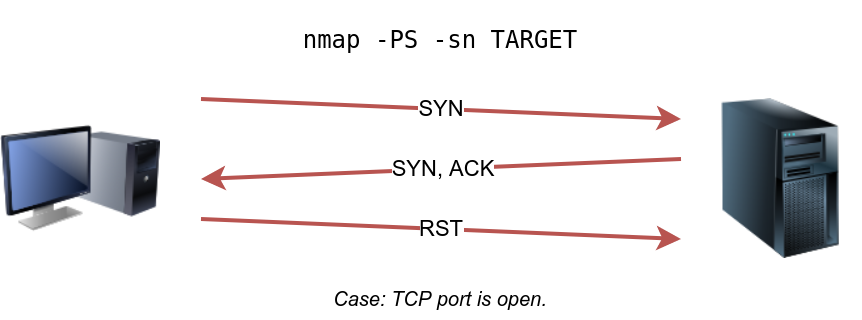
\includegraphics[width=0.7\textwidth]{SYNPack.png}
  \captionof{figure}{SYN Packet sent for Host Discovery, the user has
  root privileges.}
\end{center}
\begin{center}
  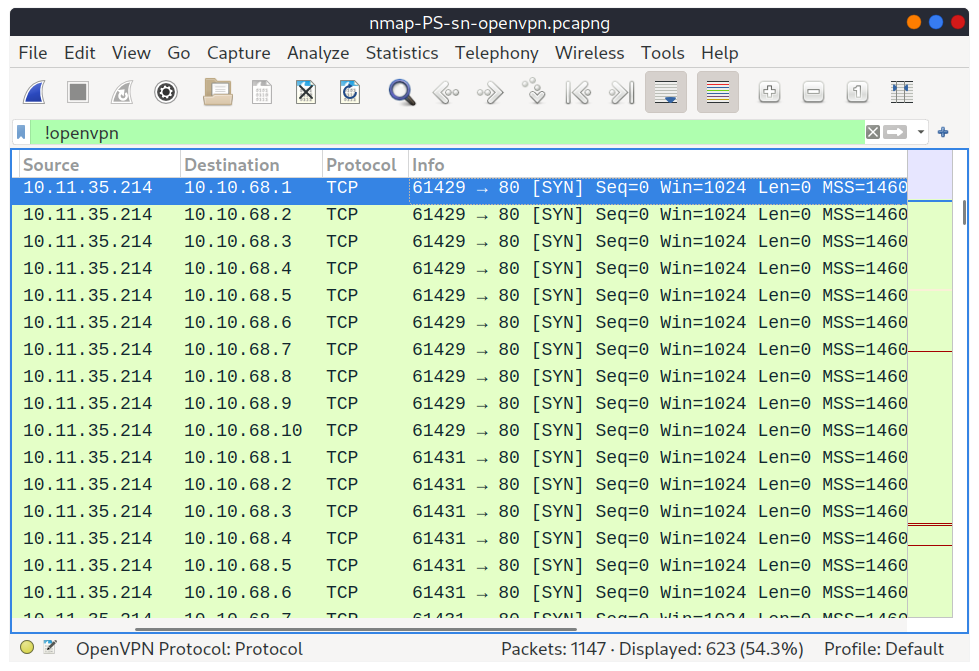
\includegraphics[width=0.7\textwidth]{HOST_SYN.png}
  \captionof{figure}{Do you notice how Nmap is sending the SYN
  packets to port 80? Twice? For each IP in the specified subnet.}
\end{center}
\subsubsection{TCP ACK Scan (-PA)}

As you have guessed, this sends a packet with an ACK flag set. Again,
by default, Nmap will send the ACK packet to port 80.

\begin{commandbox}[TCP ACK Scan (-PA)]
\begin{lstlisting}[language=bash, style=bash, basicstyle=\small\ttfamily\color{warningcolor}]
$ sudo nmap -PA -sn 10.10.68.220/24
\end{lstlisting}
\begin{lstlisting}[basicstyle=\small\ttfamily\color{kalitext}]
Starting Nmap 7.92 ( https://nmap.org ) at 2021-09-02 13:46 EEST
Nmap scan report for 10.10.68.52
Host is up (0.11s latency).
Nmap scan report for 10.10.68.121
Host is up (0.12s latency).
Nmap scan report for 10.10.68.125
Host is up (0.10s latency).
Nmap scan report for 10.10.68.134
Host is up (0.10s latency).
Nmap scan report for 10.10.68.220
Host is up (0.10s latency).
Nmap done: 256 IP addresses (5 hosts up) scanned in 29.89 seconds
\end{lstlisting}
\end{commandbox}
\begin{center}
  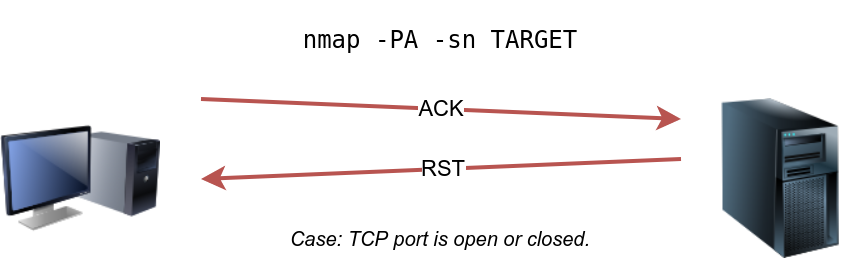
\includegraphics[width=0.7\textwidth]{ACKFlag.png}
  \captionof{figure}{TCP Packet with Ack flag set sent for Host
  Discovery, doesn't matter whether the port is open or closed}
\end{center}
\begin{center}
  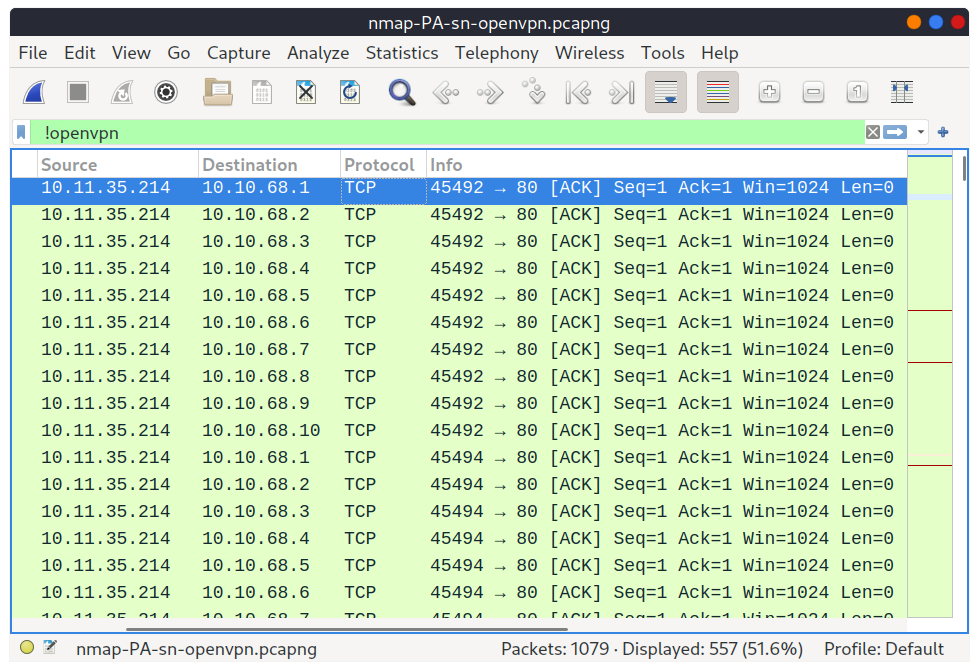
\includegraphics[width=0.7\textwidth]{HOST_ACK.png}
\end{center}
\subsubsection{UDP Scan (-PU)}

Finally, we can use UDP to discover if the host is online. Contrary
to TCP SYN ping, sending a UDP packet to an open port is not expected
to lead to any reply. However, if we send a UDP packet to a closed
UDP port, we expect to get an ICMP port unreachable packet; this
indicates that the target system is up and available, and that's
exactly why Nmap will be sending to uncommon UDP ports, so that an
ICMP destination unreachable is triggered.

\begin{commandbox}[UDP Scan (-PU)]
\begin{lstlisting}[language=bash, style=bash, basicstyle=\small\ttfamily\color{warningcolor}]
$ sudo nmap -PU -sn 10.10.68.220/24
\end{lstlisting}

\begin{lstlisting}[basicstyle=\small\ttfamily\color{kalitext}]
Starting Nmap 7.92 ( https://nmap.org ) at 2021-09-02 13:45 EEST
Nmap scan report for 10.10.68.52
Host is up (0.10s latency).
Nmap scan report for 10.10.68.121
Host is up (0.10s latency).
Nmap scan report for 10.10.68.125
Host is up (0.14s latency).
Nmap scan report for 10.10.68.134
Host is up (0.096s latency).
Nmap scan report for 10.10.68.220
Host is up (0.11s latency).
Nmap done: 256 IP addresses (5 hosts up) scanned in 9.20 seconds
\end{lstlisting}
\end{commandbox}
\begin{center}
  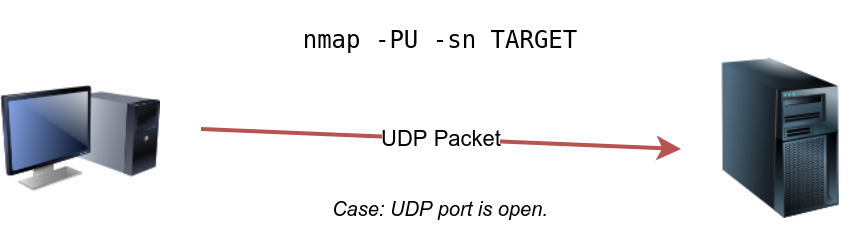
\includegraphics[width=0.7\textwidth]{UDP-Open.png}
  \captionof{figure}{UDP Packet sent for Host Discovery, port is open
  and we don't get any reply.}
\end{center}
\begin{center}
  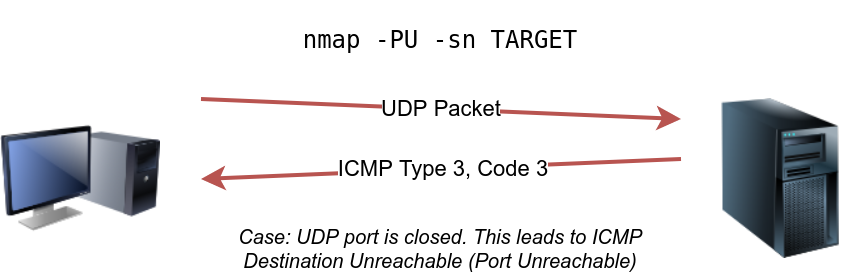
\includegraphics[width=0.7\textwidth]{UDP-Closed.png}
  \captionof{figure}{UDP Packet sent for Host Discovery, port is
  closed and we get a port unreachable packet.}
\end{center}
\begin{center}
  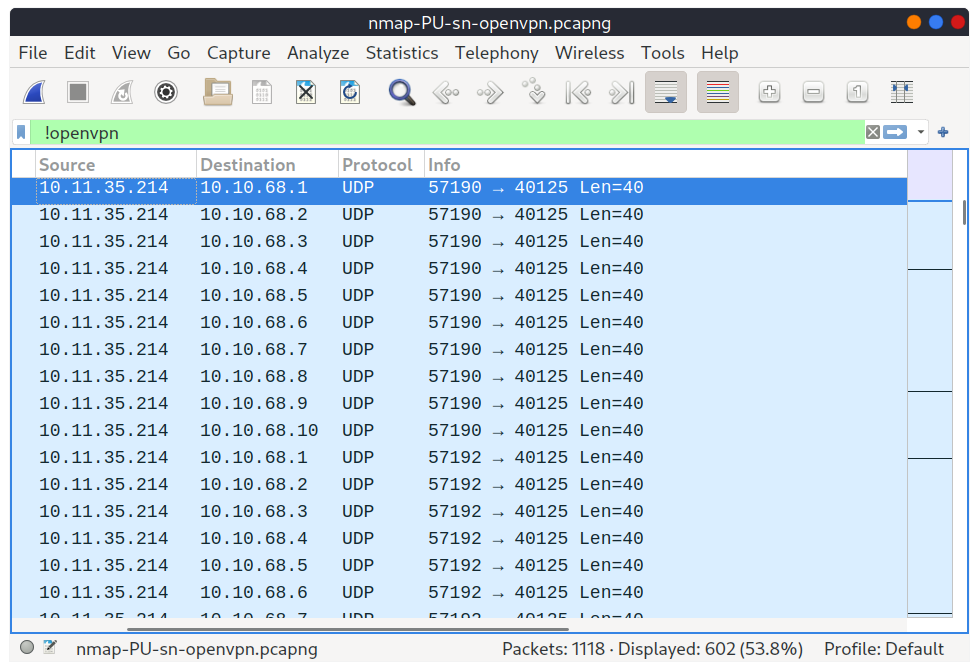
\includegraphics[width=0.7\textwidth]{HOST_UDP.png}
  \captionof{figure}{Do you notice how Nmap is sending the UDP
    packets to uncommon ports multiple times for each IP address in the
  specified subnet?}
\end{center}
\end{document}
